% $Id: circuit.tex 8323 2020-11-18 02:26:39Z mskala $

%
% MSK 013 circuit explanation
% Copyright (C) 2020  Matthew Skala
%
% This program is free software: you can redistribute it and/or modify
% it under the terms of the GNU General Public License as published by
% the Free Software Foundation, version 3.
%
% This program is distributed in the hope that it will be useful,
% but WITHOUT ANY WARRANTY; without even the implied warranty of
% MERCHANTABILITY or FITNESS FOR A PARTICULAR PURPOSE.  See the
% GNU General Public License for more details.
%
% You should have received a copy of the GNU General Public License
% along with this program.  If not, see <http://www.gnu.org/licenses/>.
%
% Matthew Skala
% https://northcoastsynthesis.com/
% mskala@northcoastsynthesis.com
%

\chapter{Circuit explanation}

The Middle Path VCO is intended to be usable both as a dual general-purpose
oscillator for two voices of subtractive synthesis in the style people
call ``East Coast,'' and as a single complex oscillator that
combines the functions of the two cores to produce a complex inharmonic
spectrum in the style called ``West Coast.''  As such, much of the design
emphasis is on versatility and making the sections work well together.

%%%%%%%%%%%%%%%%%%%%%%%%%%%%%%%%%%%%%%%%%%%%%%%%%%%%%%%%%%%%%%%%%%%%%%%%

\section{Exponential converter}

Like most analog oscillator cores, those in the MSK~013 are linearly
current-controlled, with an output frequency directly proportional to the
input current.  The exponential converter section generates control currents
for both cores, converting from the exponential voltage control standard of
Eurorack.  Some circuitry in the converter is shared between the two
oscillators in order to help them track each other as closely as possible
and to make best use of the expensive THAT320 transistor array chip. 
Although it should be as frequency-accurate in absolute terms as is normally
expected of an analog synthesizer oscillator, the real emphasis in the
design is on stability; accuracy in tracking between the two oscillators;
and ease of construction and adjustment, especially in a DIY context.

Bipolar junction transistors have a naturally exponential voltage to current
function that is surprisingly accurate.  The collector current
$I_\textrm{C}$ of a transistor in relation to the base-emitter voltage
$V_\textrm{BE}$ basically obeys the equation $I_\textrm{C} = \exp
(aV_\textrm{BE}+b)$.  But the coefficients $a$ and $b$ vary with temperature
and with the individual transistor.  To achieve accurate oscillator tuning,
we need to compensate for the variation.

The MSK~013 exponential converter uses four transistors that are built into
a single silicon chip (the THAT320 transistor array).  This chip is
specifically meant for this kind of application, and one of its selling
points is that the four transistors are made as identical as possible both
by design and by testing and selecting manufactured chips.  The fact that
all four transistors are part of a single silicon crystal keeps them at very
nearly the same temperature at all times, because silicon has a very high
thermal conductivity.  All this means that although the exponential function
of the transistors may vary from unit to unit and over time as the
temperature changes, it should at least be \emph{the same for all four
transistors}.

Then we can use two of the transistors on the chip as references, constantly
measuring the exponential curve they are producing, and apply the result of
those measurements to compensate the other two transistors (one per
oscillator) into producing the desired V/oct function.  As the temperature
changes, the performance of the transistors will change, but if they stay
close to each other and we do the measurement and compensation properly, the
overall performance of the exponential converter should not change.  The
MSK~013's use of \emph{two} reference transistors at two different current
levels eliminates the need for precision ``tempco'' components seen in more
common one-reference designs.

In keeping with the desire for all four transistors to exhibit the same
voltage/current function, every transistor in the THAT320 runs in an
environment that looks like the following.

{\centering\input{expo-q.tex}\par}

The input voltage goes through a low-resistance voltage divider that scales
it down by a factor of 3.7, in order to allow the circuit driving it to run
over a somewhat larger voltage range and be less affected by stuff like op
amp offsets.  Depending on where the transistor is being used (reference or
actually driving an oscillator) the emitter may really go to the ground
plane as shown, or it may be kept at 0V by an op amp feedback loop; and the
collector may go through the 6.8k$\Omega$ resistor to the $-$12V
power supply rail or to the current input of the oscillator core, which is
at a similar voltage.  The 6.8k$\Omega$ resistor is to limit current to a
maximum of about 1.75mA, protecting the LM13700 chips which have a maximum
rating of 2mA for control current; although such a resistor is not necessary
for protection on the reference transistors, they are given such resistors
too, to keep them running under conditions as similar as possible to the
the conditions of the oscillator-driving transistors.

The reference transistors and their driver circuits are shown in
Figure~\ref{fig:current-ref}.  These are straightforward op amp current
sources.  One end of a current-setting resistor (10k$\Omega$ R77 or
1M$\Omega$ R81) is driven by a $+$9V supply, and an op amp controls the
exponential transistor to pull the other end to 0V.  Thus the circuit is
finding a voltage to answer the question ``What input voltages does it take
to make transistors on the THAT320, at whatever temperature they are at
right now, pass 9$\mu$A and 900$\mu$A?''

\begin{figure*}
\centering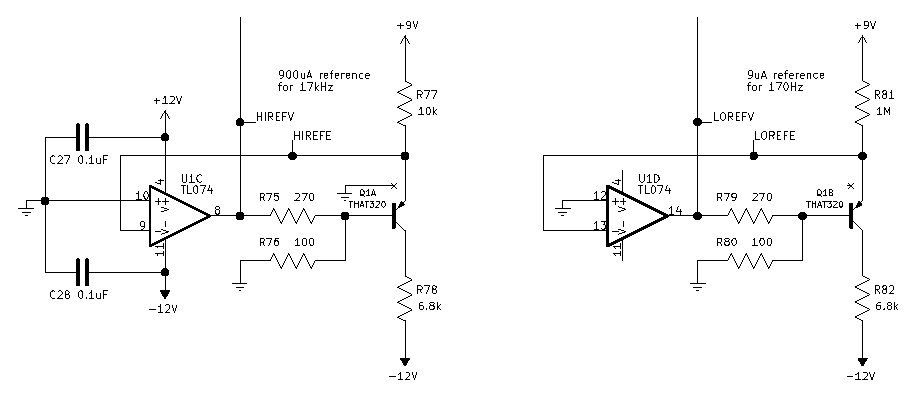
\includegraphics{current-ref}\par
\caption{Current references.}\label{fig:current-ref}
\end{figure*}

From those two voltages, we can interpolate to get the transistor voltage
for any desired current level.  For example, to get 90$\mu$A from an
oscillator-driving transistor, we would use a voltage at the midpoint of the
voltages for 9$\mu$A and 900$\mu$A.  Even if temperature changes cause the
voltages to change, as long as we track that midpoint we can expect the
output current to remain 90$\mu$A.  The voltage for either of the two
current references can provide an offset ($b$ coefficient in the
transistor's curve), and the difference between them provides the scale
factor ($a$ coefficent).  The higher current, 900$\mu$A, is two decades or
6.644 octaves from the lower current; so the voltage change on a
transistor's voltage divider input to give one octave of change in output
current, will be $1/6.644$ of the difference in reference voltage for the
two current levels.

Actually doing the interpolation requires some analog computation, which in
this design is performed by an AD633 analog multipler chip.  The AD633 is a
very expensive precision component, but it's a nearly foolproof drop-in
module that does the whole task on one chip, significantly reducing the
complexity of the circuit compared to other ways of getting a similar
effect.  A lot of the money spent on the multiplier chip is saved in labour
adjusting and debugging a more complicated exponential converter.

The AD633's basic function is that of multiplying two factors to get one
product, but both factors and the product are differential voltages, so it
actually has six pins devoted to the calculation (five inputs and one
output) and within its normal range of operation its behaviour is described
by the equation $W=Z+(X1-X2)\cdot(Y1-Y2)/10V$.  The difference in volts
between the X1 and X2 inputs, times the difference between Y1 and Y2,
divided by 10 volts, plus the voltage at Z, appears on the output W.  See
Figure~\ref{fig:expo-con} for one of the two channels of the exponential
converter using this chip.

\begin{figure*}
\centering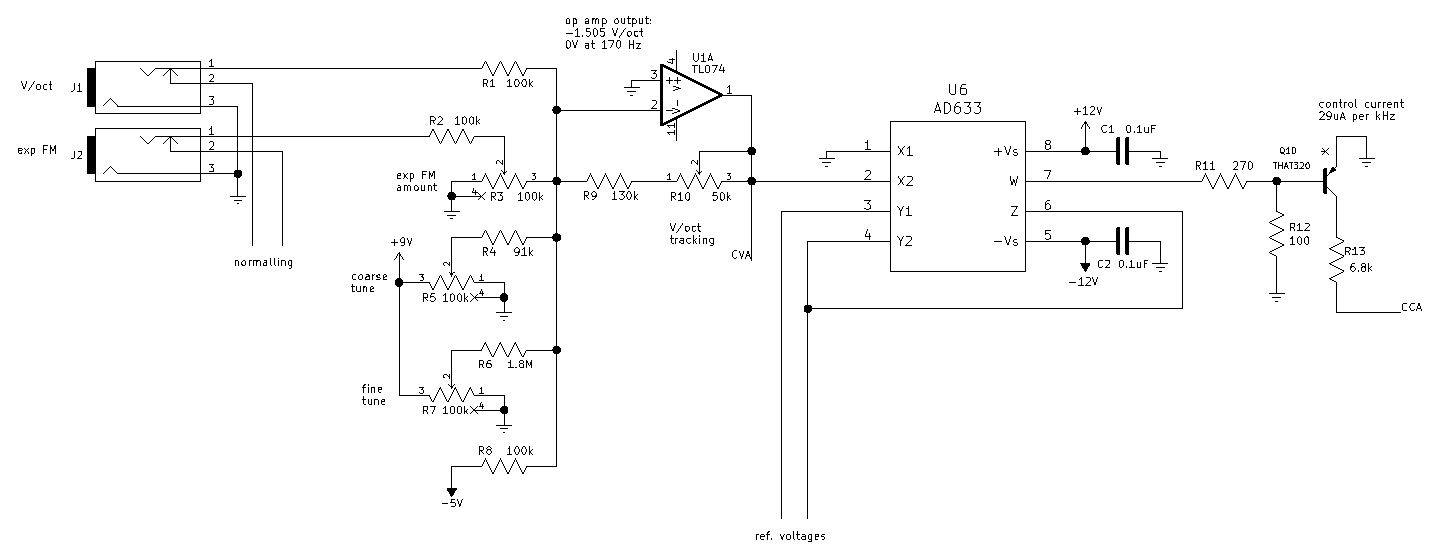
\includegraphics[width=\linewidth]{expo-con}\par
\caption{Exponential converter.}\label{fig:expo-con}
\end{figure*}

The two voltages from the current references are applied to the Y1 and Y2
inputs, so the analog multiplier is scaling its $X$ input in proportion to
the difference in voltage that it takes to increase current by a factor of
100.  That $X$ input comes from a straightforward DC mixer which combines
the settings of coarse and fine tuning knobs, the V/octave and attenuated
exponential FM control voltages, and a fixed offset (derived from a $-$5V
reference) to set the overall range of the tuning controls.  The voltage is
applied to the X2 pin with the X1 pin at ground, in order to get the right
sign on the eventual output voltage.

The output of the DC mixer is scaled to nominally $-$1.505V/octave; with the
division by 10V built into the AD633, this means each octave of control
voltage change corresponds to 0.1505 fraction of the 6.644 octaves between
the two reference currents, which does work out to one octave.  The exact
tracking can be adjusted with the trimmer in the op amp loop.

On the output side, the voltage for the 9$\mu$A current reference is also
applied to the Z input of the AD633, so when the result of the
multiplication is zero (because the op amp output was at zero), the AD633's
W output just tracks Z and the control current is 9$\mu$A.  That sets the
offset for the control circuit:  0V from the op amp corresponds to 170Hz,
and this offset automatically adjusts to follow any changes in the voltage
for 9$\mu$A that might come from temperature changes.

Some sources of error are still possible in this design, including from
inaccuracies in the AD633, temperature effects on components other than the
THAT320, and so on.  It is not the absolute most accurate exponential
converter possible.  But in practice, it works well, especially in the
musical frequnecy range of about 100Hz to 1kHz, and it requires very little
adjustment or guesswork.

%%%%%%%%%%%%%%%%%%%%%%%%%%%%%%%%%%%%%%%%%%%%%%%%%%%%%%%%%%%%%%%%%%%%%%%%

\section{Triangle cores}

The MSK~013 uses triangle-wave analog oscillator cores both as a musical
choice and to improve accuracy.  The triangle waves are close to sinusoidal,
low-harmonic waveforms suitable for shaping and modulation to add harmonics
in the sine shaper.  They also tend to track better than basic sawtooth
cores because instead of having a reset period, they have two reversals per
cycle; those reversals happen faster than a reset and are easier to control,
giving usually better accuracy from a triangle core at a given level of
circuit complexity.

The slave triangle core is shown in Figure~\ref{fig:tri-core}.  The master
is identical, minus the sync circuit.

\begin{figure*}
\centering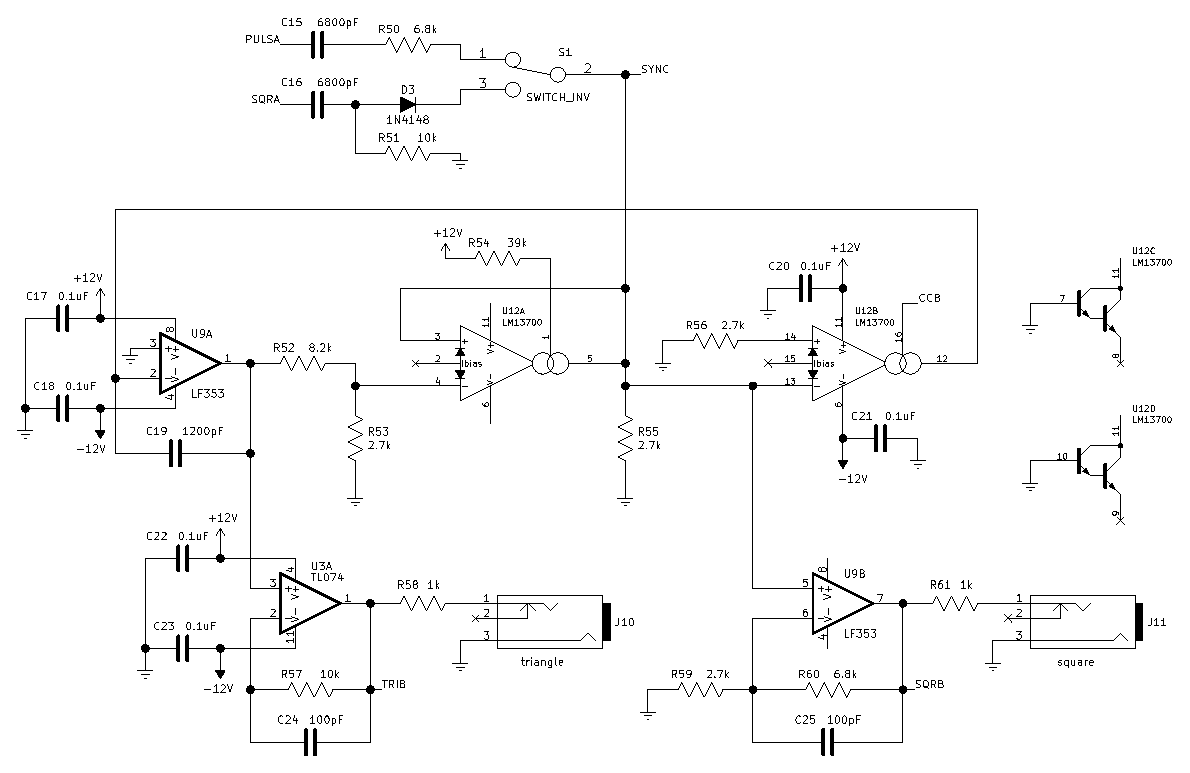
\includegraphics[width=\linewidth]{tri-core}\par
\caption{Triangle oscillator core.}\label{fig:tri-core}
\end{figure*}

Like most triangle cores, this one is a loop of three stages:  an integrator
that keeps track of the instantaneous voltage of the triangle waveform;
something (in this case a Schmitt trigger) to remember which direction the
waveform is moving and decide when to change directions; and a variable
amplifier that calculates the speed and direction the triangle voltage
should change based on pitch control input.

The LF353 op amp U9A serves as the inverting integrator.  It accumulates a
voltage in the 1200pF capacitor C19 that rises when the input to the
integrator is negative and falls when the input is positive, at a rate
proportional to the magnitude of the input voltage.  The output from this op
amp is tapped off to drive U3A, a buffer amplifier, which distributes it to
the external triangle-output jack and to the internal TRIB signal, used for
normalling the sine shaper.  Note that this op amp has an RC network of R57
and C24 in its feedback loop instead of just using a plain wire from output
to negative input; that is for stability in case of weird reactive loads
being connected to the external jack socket.

The output of the integrator also goes through a voltage divider made up of
R52 and R53 to bring it to the right level for input to U12A, an LM13700
operational transconductance amplifier (OTA) configured with positive
feedback to function as an inverting Schmitt trigger.  In a single stage
this amplifier both detects the upper and lower bounds of the triangle
waveform, and remembers the current state.

An OTA like the LM13700 works by routing the control current, in this case
coming from R54 and the positive supply, through current mirrors to shift
its direction and voltage.  For small differential input voltages it
produces a more or less linear amplifying effect, but the voltage
differences on the inputs are relatively large in this circuit, and the OTA
is basically a switch.  With the positive input at higher voltage, the OTA
sources an amount of current equal to the control current.  With the
negative input higher, it sinks the same amount.  It has a high impedance
either way, meaning that the current through the output does not depend much
on the output voltage.

Suppose the output of U12A is at positive voltage, and in particular, higher
than the scaled integrator voltage.  Then U12A's positive input is at higher
voltage, U12A sources current into R55, and that produces a positive
voltage.  The feedback loop forces U12A's output to go as high as it can go. 
A rough calculation would put the control current at 24V divided by
39k$\Omega$, which is 615$\mu$A, and then the output voltage is 2.7k$\Omega$
times that, giving $+$1.66V.  Similarly, when the output is low, the
feedback loop forces it to go as low as it can, to $-$1.66V.  In practice,
that calculation gives only an approximate value, among other reasons
because the LM13700's control input is not really quite at the negative
power rail.  The Schmitt trigger output really only swings to about
$\pm$1.5V.

That output voltage is being compared against the scaled integrator output,
as seen through the voltage divider of R52 and R53.  When the integrator
goes above about $+$6V (the nominal 1.5V Schmitt trigger threshold times the
4.03 division factor of R52 and R53), the Schmitt trigger switches to
negative output, and when the integrator goes below $-$6V, the Schmitt
trigger switches to positive output.  There is some slippage in the voltage
here too, and the voltage swing as seen at the buffered triangle output is
really more like $\pm$5.5V.  One reason is that as the integrator voltage
gets close to the threshold, the LM13700 stops functioning purely as a
switch, its output current decreases, and that reduces its output voltage,
bringing the threshold closer to the integrator voltage and making it switch
earlier.

The Schmitt trigger output also drives U9B, a non-inverting amplifier which
boosts it to about $\pm$5.5V for the ``square wave'' external output, and
U12B, which is a simple current-controlled amplifier that takes the control
current from the exponential converter and switches its direction depending
on the state of the Schmitt trigger, to apply to the integrator input.

The overall cycle of the oscillator runs as follows.  At some point the
Schmitt trigger output is positive.  U12B sinks current, in an amount
determined by the exponential converter.  That causes the voltage output of
U9B to rise.  When it reaches about $+$5.5V, the Schmitt trigger switches to
negative output.  Then U12B sources current instead of sinking it, causing
the voltage output of U9B to fall.  When it reaches $-$5.5V, the Schmitt
trigger switches to positive again and the cycle can repeat.  So the
integrator output is a triangle wave, bouncing between $\pm$5.5 with a slope
determined by the current from the exponential converter, and the Schmitt
trigger output is a square wave, positive when the triangle is rising and
negative when it is falling.  The speed of the entire cycle is proportional
to the current from the exponential converter, and that proportionality is
quite exact over at least the entire audio frequency range, 20Hz to 20kHz.

%%%%%%%%%%%%%%%%%%%%%%%%%%%%%%%%%%%%%%%%%%%%%%%%%%%%%%%%%%%%%%%%%%%%%%%%

\section{Sync}

The switch S1, shown near the top of Figure~\ref{fig:tri-core}, selects
either of two simple sync circuits, or no sync in the centre ``off''
position.

In \emph{firm} sync mode, S1 selects C15 and R50, which form a simple
high-pass filter.  The internal PULSA signal, representing the pulse shaper
output of the master oscillator, gets coupled through these components to
the Schmitt trigger of the slave oscillator.  When the master pulse output
goes high, a current spike is applied across R55, forcing the Schmitt
trigger into the high state and the slave oscillator into the rising state
of its cycle.  Similarly, when the master pulse output goes low, a current
spike in the other direction passes through C15 and R50, forcing the slave
oscillator Schmitt trigger into the low state.  I call this firm sync
because it has a relatively strong effect on the slave oscillator's phase,
making it lock quickly to the master, but it does not reset the integrator
to a fixed voltage immediately like the true hard sync typical of saw-core
oscillators.  The exact spectral effect of firm sync will vary depending on
the pulse width (and pulse width modulation) of the master oscillator.

In \emph{soft} sync mode, the master square wave (not pulse) output goes
through C16, R51, and D3.  The diode allows pulses to pass only on the
rising edge of the square wave.  The resistor allows the capacitor to
recharge on the opposite pulse edge.  Here the slave is only switched to
the rising state once per cycle of the master, so it takes longer to lock.

In either mode, because the sync pulses are applied directly to the Schmitt
trigger output of the slave oscillator core and that is also the source for
the slave oscillator's square wave output, the sync pulses will appear in
the square wave, often pushing its voltage outside the usual range of
approximately $\pm$5.5V.  Sync pulses can also hold the slave oscillator in
a given state briefly even when the integrator voltage would normally switch
its direction; as a result, the slave triangle output can also go out of its
normal voltage range when in sync mode.

%%%%%%%%%%%%%%%%%%%%%%%%%%%%%%%%%%%%%%%%%%%%%%%%%%%%%%%%%%%%%%%%%%%%%%%%

\section{Pulse and sawtooth shapers}

\begin{figure*}
\centering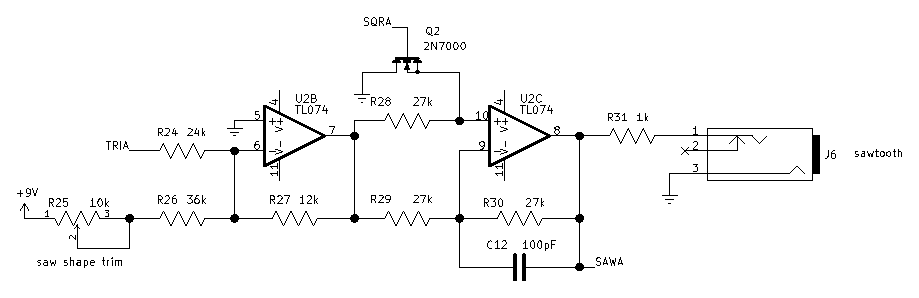
\includegraphics{saw-shaper}\par
\vspace{18pt}
\begin{tikzpicture}[>=Stealth]
  \draw[->,thick] (-0.5,0) -- (12.5,0);
  \draw[->,thick] (-0.5,-3) -- (12.5,-3);
  \draw[->,thick] (-0.5,-6) -- (12.5,-6);
  \draw[->,thick] (-0.5,-9) -- (12.5,-9);
  \draw[->,thick] (0,-1.3) -- (0,1.3);
  \draw[->,thick] (0,-4.3) -- (0,-1.7);
  \draw[->,thick] (0,-7.3) -- (0,-4.7);
  \draw[->,thick] (0,-10.3) -- (0,-7.7);
  \node at (-1.5,0) {\textsf{TRIA}};
  \node at (-1.5,-3) {\textsf{SQRA}};
  \node at (-1.5,-6) {\textsf{U2B}};
  \node at (-1.5,-9) {\textsf{U2C}};
  \draw[ultra thick] (-0.2,-0.2) -- (1,1) -- (3,-1) -- (5,1)
    -- (7,-1) -- (9,1) -- (11,-1) -- (12.2,0.2);
  \draw[ultra thick] (-0.2,-2) -- (1,-2) -- (1,-4) -- (3,-4) -- (3,-2)
    -- (5,-2) -- (5,-4) -- (7,-4) -- (7,-2) -- (9,-2) -- (9,-4)
    -- (11,-4) -- (11,-2) -- (12.2,-2);
  \draw[ultra thick] (-0.2,-6.4) -- (1,-7) -- (3,-6) -- (5,-7)
    -- (7,-6) -- (9,-7) -- (11,-6) -- (12.2,-6.6);
  \draw[ultra thick] (-0.2,-8.6) -- (1,-8) -- (1,-10) -- (5,-8) -- (5,-10)
    -- (9,-8) -- (9,-10) -- (12.2,-8.4);
  \draw[ultra thick] (3,-8.9) -- (3,-9.1);
  \draw[ultra thick] (7,-8.9) -- (7,-9.1);
  \draw[ultra thick] (11,-8.9) -- (11,-9.1);
\end{tikzpicture}\par
\caption{Sawtooth shaper with its waveforms.}\label{fig:saw-shaper}
\end{figure*}

Each oscillator core has a sawtooth shaper, which converts the triangle and
square wave outputs from the core into a sawtooth waveform.  The sawtooth
shaper from the master oscillator is shown in Figure~\ref{fig:saw-shaper};
the slave's is just the same.

The op amp U2B is set up as an inverting amplifier with a gain (determined
by the ratio of R27 and R24) of $-$0.5.  There is also a negative offset
created by current from the $+$9V reference through R25 and R26; so the
triangle wave which comes in at nominally $\pm$5.5V is shifted and scaled to
cover the range $-$5.5V to 0V.

The op amp U2C is either a unity-gain amplifier or an inverter, depending on
the state of Q2.  This MOSFET functions as a switch:  with the square wave
high, the MOSFET conducts, holding the positive input of U2C at 0V.  In this
state, U2C functions as an inverter with gain $-$1, as set by R29 and R30. 
When the square wave goes low, Q2 turns off.  Then the positive input of U2C
stays at the output voltage of U2B; and in order to keep the negative input
at that same voltage, U2C must also track the output voltage of U2B; the
amplifier has gain $+$1.

Now, consider the progress of an oscillator cycle, starting at the high peak
of the triangle wave.  In the falling phase, the triangle goes from $+$5.5V
down to $-$5.5V and the square wave is low.  The output of U2B (inverted,
scaled, and shifted) goes from $-$5.5V up to 0V.  The MOSFET is turned off,
so U2C acts as a unity-gain buffer for the U2B voltage, and the sawtooth
output rises from $-$5.5V to 0V.  Then the triangle reverses direction,
rising from $-$5.5V up to $+$5.5V.  The output of U2B goes from 0V down to
$-$5.5V.  The square wave is high now, turning on Q2, and U2C functions as
an inverter; the sawtooth output continues rising from 0V up to $+$5.5V. 

The waveforms in Figure~\ref{fig:saw-shaper} illustrate the operation of the
shaper.  There is usually a small glitch when the sawtooth crosses zero
because of timing inaccuracy between the triangle and square signals, and
the nonzero time required to switch between the inverting and noninverting
configuations of U2C.  The offset trimmer R25 can be adjusted to minimize
this glitch and line up the two halves of the sawtooth as accurately as
possible.

\begin{figure*}
\centering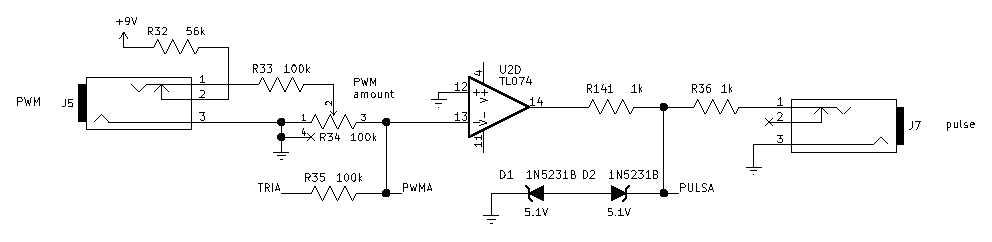
\includegraphics{pulse-shaper}\par
\caption{Pulse shaper.}\label{fig:pulse-shaper}
\end{figure*}

The pulse shaper for the master oscillator is shown in
Figure~\ref{fig:pulse-shaper}; that for the slave is just the same.  This
circuit is basically just an op amp working as a comparator, with its
support components.  Many sources advise against using op amps to compare
voltages instead of special-purpose comparator ICs, among other reasons
because an op amp driven to its maximum or minimum voltage can ``saturate''
and then take longer to come out of that state than its usual response time. 
But after testing several alternatives, it really seems the straightforward
op amp as comparator is the best design for this circuit in this particular
application.  With the specified TL074 chip, the response time coming out of
saturation is more than fast enough for even the highest audio frequencies.

The reference voltage from J5, either an input PWM signal or the
normalization voltage, is attenuated by R33 and R34 and applied to the
negative input of the op amp.  So is the oscillator triangle output, through
R35.  If the average of these two voltages is above zero, the op amp output
goes strongly positive; if below, it goes negative.  Then D1 and D2 serve to
clip the voltage to approximately $\pm$5.6V.  The resistor R141 limits the
current from the op amp output, and R26 limits the current through the
output jack (especially in the case where somebody patches it into a power
supply).

%%%%%%%%%%%%%%%%%%%%%%%%%%%%%%%%%%%%%%%%%%%%%%%%%%%%%%%%%%%%%%%%%%%%%%%%

\section{Quadrature sine shaper}

The Middle Path VCO's quadrature sine shaper is probably the most innovative
part of the module, and key to its unique sound and feature set.  There is a
lot going on in this circuit, but it can be thought of as a straightforward
evolution from a simple, familiar analog building block:  the differential
pair.

Here's a differential pair of NPN transistors.

{\centering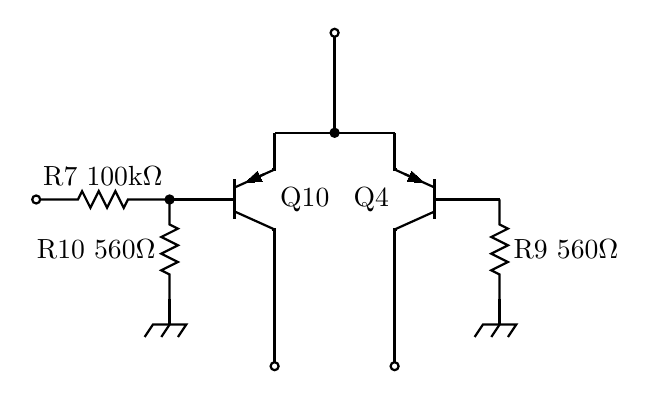
\begin{tikzpicture}[scale=2.54]
% dpic version 2014.Jan.01 option -g for TikZ and PGF 1.01
\ifx\dpiclw\undefined\newdimen\dpiclw\fi
\global\def\dpicdraw{\draw[line width=\dpiclw]}
\global\def\dpicstop{;}
\dpiclw=0.8bp
\dpiclw=0.8bp
\dpicdraw[fill=black](0,0) circle (0.007874in)\dpicstop
\dpicdraw (0,0)
 --(-0.3,0)\dpicstop
\dpicdraw (-0.3,0)
 --(-0.3,-0.1835)
 --(-0.31107,-0.1835)\dpicstop
\dpicdraw (-0.3,-0.667)
 --(-0.3,-0.4835)
 --(-0.31107,-0.4835)\dpicstop
\dpicdraw (-0.5,-0.2335)
 --(-0.5,-0.4335)\dpicstop
\dpicdraw (-0.625,-0.3335)
 --(-0.5,-0.3335)\dpicstop
\dpicdraw (-0.3,-0.1835)
 --(-0.5,-0.2735)\dpicstop
\dpicdraw (-0.35,-0.206)
 --(-0.374007,-0.216803)\dpicstop
\filldraw[line width=0bp](-0.385406,-0.191472)
 --(-0.45,-0.251)
 --(-0.362608,-0.242134) --cycle
\dpicstop
\dpicdraw (-0.3,-0.4835)
 --(-0.5,-0.3935)\dpicstop
\draw (-0.3,-0.3335) node[right=-1.5bp]{$ \textrm{Q10}$};
\dpicdraw (0,0)
 --(0.3,0)\dpicstop
\dpicdraw (0.3,0)
 --(0.3,-0.1835)
 --(0.31107,-0.1835)\dpicstop
\dpicdraw (0.3,-0.667)
 --(0.3,-0.4835)
 --(0.31107,-0.4835)\dpicstop
\dpicdraw (0.5,-0.2335)
 --(0.5,-0.4335)\dpicstop
\dpicdraw (0.625,-0.3335)
 --(0.5,-0.3335)\dpicstop
\dpicdraw (0.3,-0.1835)
 --(0.5,-0.2735)\dpicstop
\dpicdraw (0.35,-0.206)
 --(0.374007,-0.216803)\dpicstop
\filldraw[line width=0bp](0.362608,-0.242134)
 --(0.45,-0.251)
 --(0.385406,-0.191472) --cycle
\dpicstop
\dpicdraw (0.3,-0.4835)
 --(0.5,-0.3935)\dpicstop
\draw (0.3,-0.3335) node[left=-1.5bp]{$ \textrm{Q4}$};
\dpicdraw (0,0)
 --(0,0.5)\dpicstop
\dpicdraw[fill=white](0,0.5) circle (0.007874in)\dpicstop
\dpicdraw (-0.3,-0.667)
 --(-0.3,-1.167)\dpicstop
\dpicdraw[fill=white](-0.3,-1.167) circle (0.007874in)\dpicstop
\dpicdraw (0.3,-0.667)
 --(0.3,-1.167)\dpicstop
\dpicdraw[fill=white](0.3,-1.167) circle (0.007874in)\dpicstop
\dpicdraw (-0.625,-0.3335)
 --(-0.825,-0.3335)\dpicstop
\dpicdraw[fill=black](-0.825,-0.3335) circle (0.007874in)\dpicstop
\dpicdraw (-0.825,-0.3335)
 --(-0.825,-0.4585)
 --(-0.783333,-0.479333)
 --(-0.866667,-0.521)
 --(-0.783333,-0.562667)
 --(-0.866667,-0.604333)
 --(-0.783333,-0.646)
 --(-0.866667,-0.687667)
 --(-0.825,-0.7085)
 --(-0.825,-0.8335)\dpicstop
\draw (-0.866667,-0.5835) node[left=-1.5bp]{$ \textrm{R10 560}\Omega$};
\dpicdraw (-0.825,-0.8335)
 --(-0.825,-0.9585)\dpicstop
\dpicdraw (-0.783333,-1.021)
 --(-0.741667,-0.9585)
 --(-0.908333,-0.9585)
 --(-0.95,-1.021)\dpicstop
\dpicdraw (-0.825,-0.9585)
 --(-0.866667,-1.021)\dpicstop
\dpicdraw (-0.825,-0.3335)
 --(-1.0335,-0.3335)
 --(-1.054333,-0.375167)
 --(-1.096,-0.291833)
 --(-1.137667,-0.375167)
 --(-1.179333,-0.291833)
 --(-1.221,-0.375167)
 --(-1.262667,-0.291833)
 --(-1.2835,-0.3335)
 --(-1.492,-0.3335)\dpicstop
\draw (-1.1585,-0.291833) node[above=-1.5bp]{$ \textrm{R7 100k}\Omega$};
\dpicdraw[fill=white](-1.492,-0.3335) circle (0.007874in)\dpicstop
\dpicdraw (0.625,-0.3335)
 --(0.825,-0.3335)\dpicstop
\dpicdraw (0.825,-0.3335)
 --(0.825,-0.4585)
 --(0.866667,-0.479333)
 --(0.783333,-0.521)
 --(0.866667,-0.562667)
 --(0.783333,-0.604333)
 --(0.866667,-0.646)
 --(0.783333,-0.687667)
 --(0.825,-0.7085)
 --(0.825,-0.8335)\dpicstop
\draw (0.866667,-0.5835) node[right=-1.5bp]{$ \textrm{R9 560}\Omega$};
\dpicdraw (0.825,-0.8335)
 --(0.825,-0.9585)\dpicstop
\dpicdraw (0.866667,-1.021)
 --(0.908333,-0.9585)
 --(0.741667,-0.9585)
 --(0.7,-1.021)\dpicstop
\dpicdraw (0.825,-0.9585)
 --(0.783333,-1.021)\dpicstop
\end{tikzpicture}
\par}

The current sink at the bottom draws a fixed amount of current through the
two transistors combined.  Excluding whatever flows through the bases (which
should be negligible if the transistors have reasonably high gain), the sum
of the two collector currents of the transistors will be forced equal to the
constant current of the current sink.  The emitters of the transistors,
which are joined, will naturally float to whatever voltage it takes to make
that work.

But the split between the two transistors, how much of the total current
goes to which transistor, will be determined by the difference in voltages
applied to their bases.  If the base voltages are equal, the current should
split 50/50.  If one base is about 18mV more positive (assuming silicon
transistors at room temperature), then the current through that transistor
will be twice as much as the current through the other transistor; that is,
two thirds of the total.  Note that each transistor's share is an
exponential function of its base voltage relative to the other transistor.

The split depends on the \emph{difference} in base
voltages but not on the \emph{absolute value} of the base voltages; if both
bases go up or down by the same amount within the limits of the circuit, the
proportional split between the two transistors does not change.  The
proportional split also should not change if the current sink's current
changes; both transistor collector currents scale in proportion to the
total.  Depending on the application, it's expected that some stage further
downstream will capture the currents flowing through either or both
collectors and do something useful with the result.

The basic differential pair is commonly seen at the input of an op amp
circuit.  It can also be used to build a VCA or multiplying circuit:  one
factor to be multiplied gets applied as a base voltage and the other is used
to control the current sink, possibly through a current mirror.

What if we generalize the circuit to use more than two transistors?  All
emitters will be connected together with a constant current sink drawing a
fixed current through the collection of transistors.  The current into the
current sink splits more than two ways, some flowing through each
transistor.  The basic principle remains the same as in the two-transistor
differential pair: the sum of all the collector currents, excluding
negligible currents through the bases, must be equal to the current-sink
current, and the joined emitters of all the transistors will float to
whatever voltage it takes to make that equation true.  And then the
difference in base voltages will determine the proportional split among the
transistors; whichever transistor has the highest base voltage gets the most
current, and others get less, in proportion to an exponential function of
how much their own base voltages are below the highest.

If we could give just one transistor a significantly higher base voltage
than the others, that transistor would get almost all the current-sink
current.  If we gave relatively high base voltages to \emph{two}
transistors, they would split the current, in proportions determined by any
difference between their base voltages.  In general, the one or more
transistors with the highest base voltages will split the current and any
others with significantly lower base voltages will be turned off, passing
effectively no current.  Barrie Gilbert patented a well-known sine
waveshaping circuit based on this principle (US Patent \#4,475,169A, now
long since expired): a differential ``pair'' generalized to use more than
two transistors, with the current split among the transistors used to
smoothly interpolate between the peaks of the desired voltage function.

\begin{figure*}
\centering\input{parabolas.tex}\par
\caption{Transistor base voltages in the sine shaper.}\label{fig:parabolas}
\end{figure*}

Consider the resistor network shown in Figure~\ref{fig:parabolas}.  It is
assumed that driver amplifiers not shown apply an input voltage to one
end of the network, and the opposite of the input voltage to the other end. 
Current flows from one end to the other, through a chain of resistors of
relatively low value, so that effect alone should cause the voltages along
the chain to interpolate linearly from the input voltage to its negative. 
But there are also resistors of relatively high value pulling up the
voltages along the chain toward $+$12V.  Near the ends, the low impedance
from the driver circuits prevents those pull-ups from having much effect. 
But toward the centre, there is less influence from the drivers and the
pull-ups are more able to raise the voltage.

The overall behaviour of this network (illustrated for three different input
voltages in the figure) is that the voltages at different points along the
chain will approximate a parabola or quadratic function, with a peak that
shifts left and right, toward one end of the chain or the other, according
to the input voltage.

In the Gilbert sine shaper, the voltages from this kind of network are
applied to the bases of transistors in a many-transistor generalized
differential pair.  At zero input, the peak in voltages is in the middle of
the chain; as the input goes positive or negative, the peak moves forward
and backward along the chain.  Transistors at or near the peak split up the
current; transistors further away from the peak are turned off.

The next step is that in Gilbert's version of the circuit, the current
outputs from alternate transistors are \emph{summed} by connecting them
together.  All the even-numbered transistors drive one current output, and
all the odd-numbered transistors drive the other.  And then another
differential amplifier computes the difference between the even-transistor
and odd-transistor currents.

Think about what happens as the input voltage increases.  The peak in base
voltages moves along the chain.  When it hits an even-numbered transistor,
that transistor carries most of the current-sink current, and so the
even-transistor group is carrying more current than the odd-transistor
group and the difference is maximized in one direction (let's say positive). 
As the peak continues moving, it will hit an odd-numbered transistor.  Then
that transistor carries most of the current, so the odd-transistor group
carries most of the current, and the difference is now maximized in the
other direction (let's say negative).  The output of the Gilbert shaper
switches back and forth several times as the input voltage moves across its
range.

The peak of the base voltages doesn't really activate just one transistor at
a time; other transistors on either side of the peak will always also be
conducting to some extent.  That reduces the overall output voltage because
the difference between the even and odd groups will never be overwhelming;
but it also means that the interpolation between positive and negative peaks
is smooth.  The cool thing is that the math works out such that within
reasonable limits, the interpolation is not only smooth but
\emph{sinusoidal}.  Within the limits of the circuit, for a number of cycles
that is determined by the number of transistors used, and subject to
scaling, the Gilbert sine shaper computes something very close to
$V_\textrm{out} = \sin V_\textrm{in}$.

The \emph{quadrature} sine shaper used in the Middle Path VCO takes the sine
shaping circuit another step further, by grouping the transistors into four
groups instead of two.  As far as I know, this idea is original with me,
although it's sufficiently obvious that I wouldn't be too surprised to hear
someone else had thought of it earlier.  The core of the quadrature sine
shaper circuit is shown in Figure~\ref{fig:sh-core}.

In the quadrature shaper, there are twelve transistors in the chain,
assigned to four groups in a rotating pattern.  All the collectors for
Group~1, being the first, fifth, and ninth transistors along the chain, are
connected together, so the collector currents for those transistors add up,
appear as a voltage across R116, and then a unity-gain op amp buffers the
resulting voltage to produce an internal signal called GROUP1.  The
remaining transistors are similarly gathered into groups of three to
generate summed and buffered voltage signals.

Note that GROUP1 and GROUP3 \emph{together} cover all the odd-index
transistors (counting the first transistor on the left as index 1), and
GROUP2 and GROUP4 together cover all the even-index transistors.  So if we
compute the sum of the GROUP1 and GROUP3 voltages, minus the GROUP2 and
GROUP4 voltages, we end up with just the odd transistors minus the even
transistors and that is the same result we could get from the basic
one-output Gilbert sine shaper.  The op amp U5C does that sum and difference
calculation, with appropriate scaling.

\noindent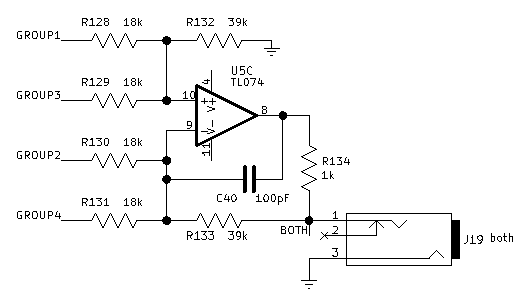
\includegraphics[width=\linewidth]{sh-outmix-both}

But GROUP1 and GROUP3 can also be considered separately.  The odd-index
transistors are all assigned to one of those two groups, but they
alternate between them:  the transistor at index 1 is in GROUP1, then the
one at index 3 is in GROUP3, then the one at index 5 is in GROUP1, and so
on.  GROUP1 and GROUP3 can be said to be the odd and even transistors within
the larger ``odd'' group.  Similarly, GROUP2 and GROUP4 are the odd and even
transistors within the larger ``even'' group.

\begin{sidewaysfigure}
\centering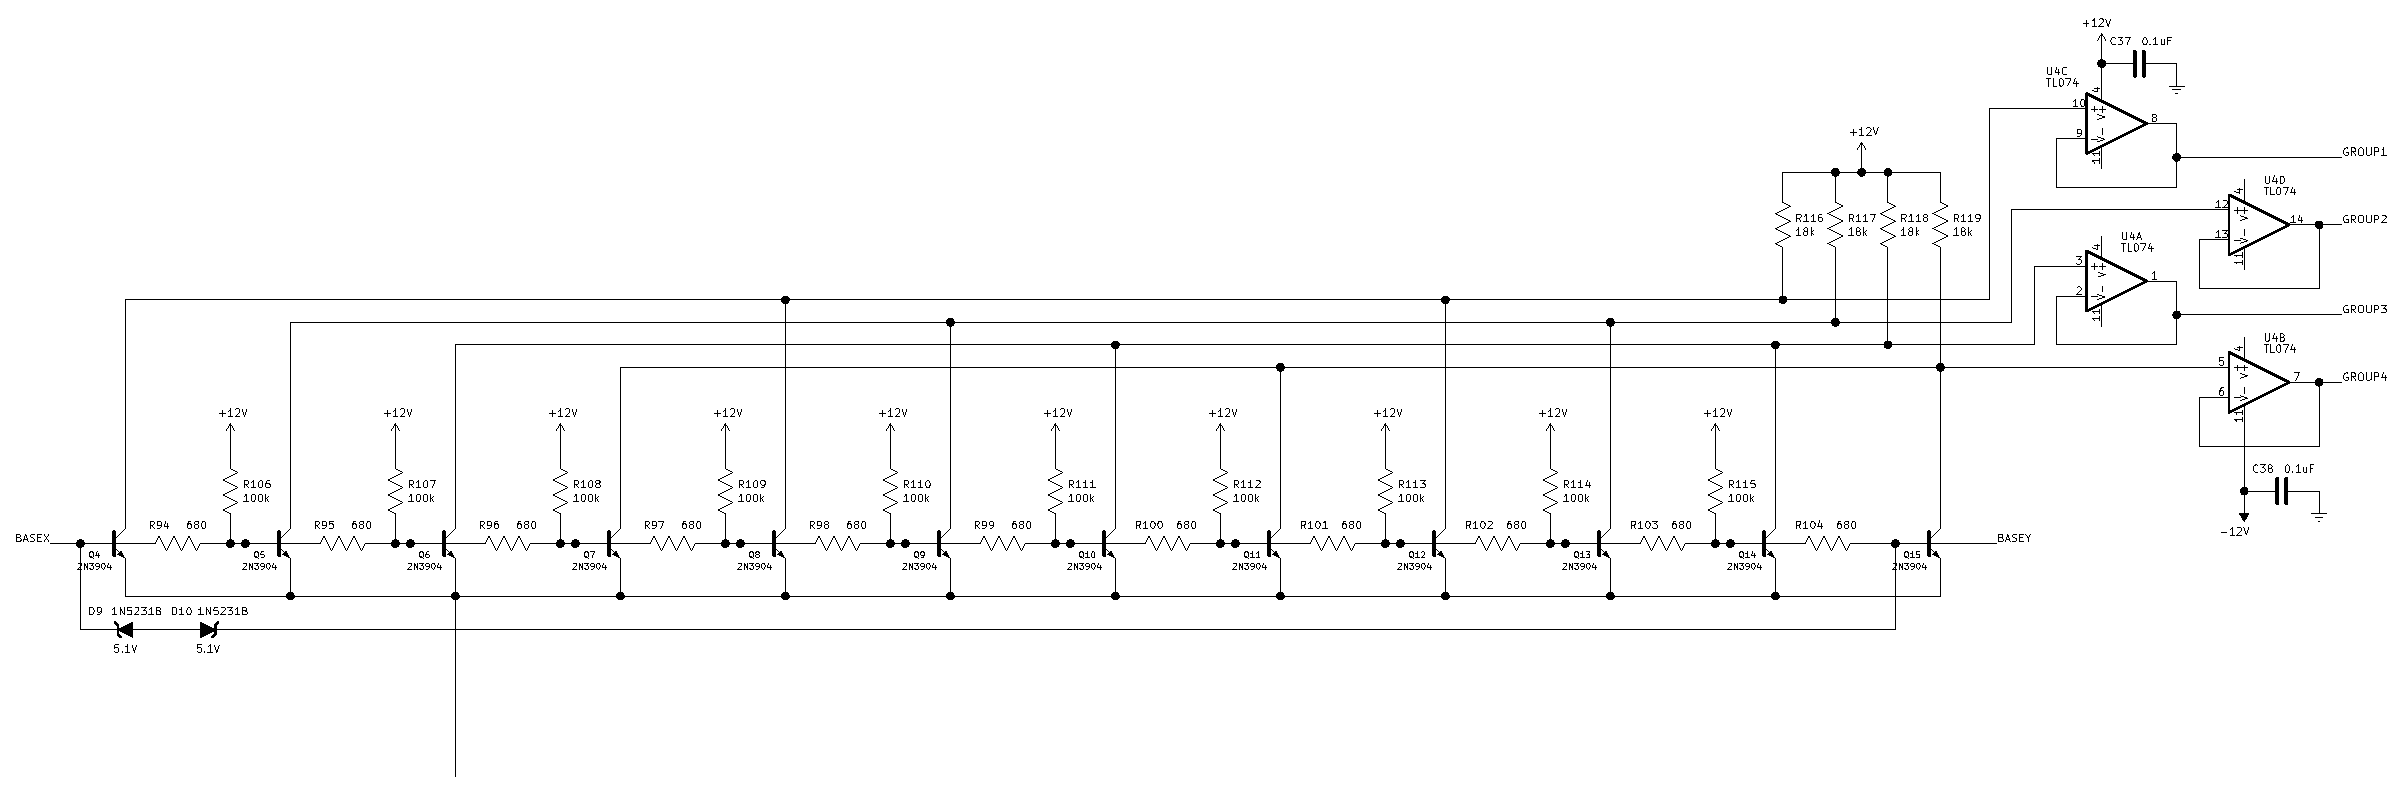
\includegraphics[width=\linewidth]{sh-core}\par
\caption{Quadrature sine shaper core.}\label{fig:sh-core}
\end{sidewaysfigure}

So we can get two more sine-function outputs by taking the difference
between GROUP1 and GROUP3, and the difference between GROUP2 and GROUP4. 
The op amp U5D does this calculation for GROUP1 and GROUP3; I don't show U5B
here but it works the same way on GROUP2 and GROUP4.  These are the module
``sin'' and ``cos'' outputs.  They each have three cycles along the length
of the transistor chain, because there are three transistors in each group;
but because the cyclic assignment of transistors to groups is shifted by one
quarter cycle (one transistor position) between the two outputs, their sine
functions are 90$^\circ$ out of phase.  The frequency of these sine
functions, relative to input voltage, is half that seen on the ``both''
output because the ``both'' output is using six transistors per group.

\pagebreak

Here is the mixer for the ``sin'' output; the mixer for ``cos'' is similar,
but uses the other two group signals.

\noindent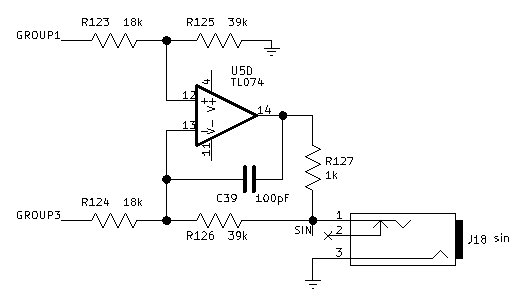
\includegraphics[width=\linewidth]{sh-outmix-sin}

The cyclic assignment of transistors to four groups is the key concept in
the quadrature sine shaper.  There are just a few other things to mention in
the shaper circuit and they are fairly straightforward.  Note the clipping
diodes D9 and D10, from the transistor at one end of the chain to the other. 
Those are to prevent reverse breakdown in the transistors.  Remember that
the voltage on the joined emitter of all the transistors will always be
basically one diode drop lower than the peak base voltage along the chain. 
At an extreme high or low input voltage, the peak is driven all the way to
one end of the chain, and will be basically equal to the absolute value of
the input voltage.  The other end of the chain gets the negative of that; so
the transistor there will be seeing twice the input voltage, minus one diode
drop, in reverse across its base-emitter junction.

The 2N3904 transistors used here are only rated for 6.0V in that direction;
more voltage and they can be damaged.  Many other common transistors have an
even lower breakdown voltage, which is why I specified 2N3904 in particular
for these.  Higher-gain transistors which might usually be considered higher
``quality'' are likely to have low breakdown voltages because gain and
breakdown voltage are both determined largely by the level of emitter
doping.  Increasing one tends to decrease the other.

The diodes D9 and D10 protect the transistors because on out-of-range input
voltages they will conduct and clip the voltage difference seen by the ends
of the transistor chain to about 5.7V; the maximum reverse voltage on the
transistor junctions is then about 5.1V and safely within the transistor
specifications.

The input voltage range needed to cover the whole transistor chain is
basically proportional to the number of transistors and the size of a diode
drop.  In the original Gilbert design it's not the usual practice to have so
many transistors as I am using here, so the input voltage can be scaled down
more and still cover the whole chain.  In the quadrature design, there are
basically twice as many transistors needed for the same number of sine
cycles, and that means scaling the input voltages larger and coming closer
to the reverse-breakdown limits of the transistors.

The current sink is a straightforward design in which an op amp drives a
transistor base to keep the voltage across a resistor constant.

{\centering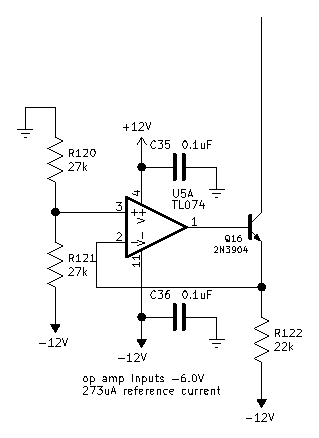
\includegraphics{sh-csink}\par}

Finally, the shaper input mixer (Figure~\ref{fig:sh-inmix}) is a
conventional inverting op amp design with a second inverting op amp to
compute the voltage for the other end.  Note both ends have 680$\Omega$
resistors to limit the current when the clipping diodes turn on.

\begin{figure*}
\centering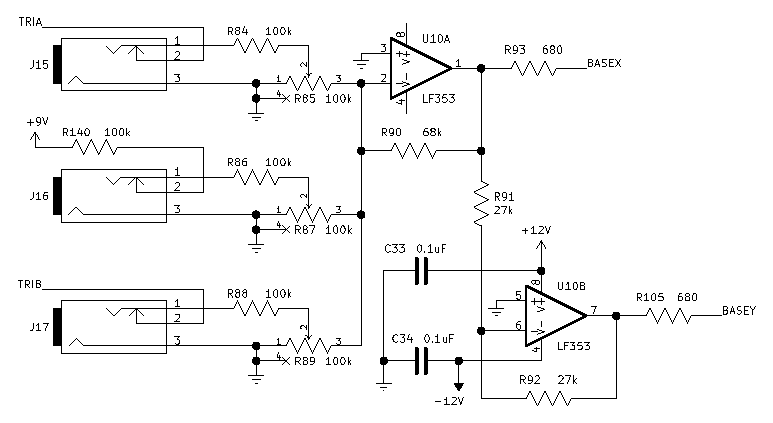
\includegraphics{sh-inmix}\par
\caption{Quadrature sine shaper input mixer.}\label{fig:sh-inmix}
\end{figure*}
